\section{現状の課題}
\subsection{アンケート結果による現状の分析}
土佐山田町の地域情報の入手状況と地域SNSに必要な情報及び機能についてアンケートを実施した.アンケートは土佐山田町に住む10代から50代の男女に実施した.

\subsubsection{地域のイベントやお店の情報をどのくらいチェックしていますか?}
\begin{figure}[H]
    \centering
    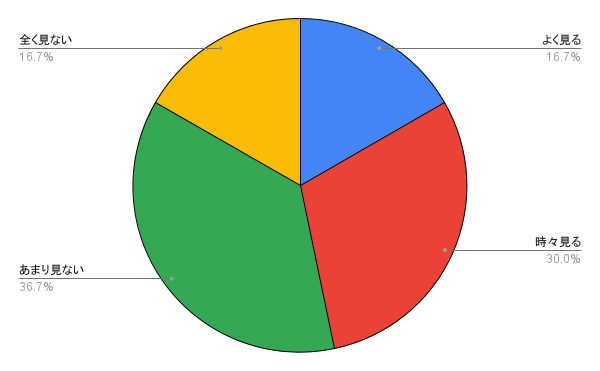
\includegraphics[width=0.5\linewidth]{fig125/Q1.png}
    \caption{地域情報等を見る頻度}
    \label{fig:Q1}
\end{figure}
図\ref{fig:Q1}より,5割程度の人が土佐山田町に関する情報をあまり見ない,全く見ないと回答している.

\subsubsection{地域情報は普段どこから得ていますか?(複数回答可)}
\begin{figure}[H]
    \centering
    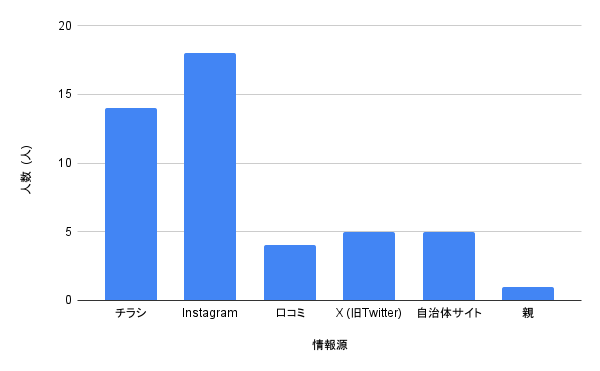
\includegraphics[width=0.5\linewidth]{fig125/Q3.png}
    \caption{地域情報の入手先}
    \label{fig:Q3}
\end{figure}
図\ref{fig:Q3}より,地域情報は主にInstagramやチラシから得ていることが分かった.

\subsubsection{どんな情報を地域SNSで見たいですか?(複数回答可)}
\begin{figure}[H]
    \centering
    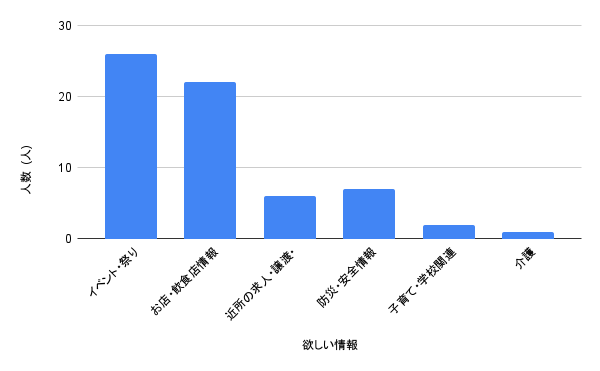
\includegraphics[width=0.5\linewidth]{fig125/Q4.png}
    \caption{見たい地域情報}
    \label{fig:Q4}
\end{figure}
図\ref{fig:Q4}より,地域SNSがあるならば,イベント情報や飲食店の情報を入手したい人が多いことが分かった.

\subsubsection{どんな機能があれば使いたいと思いますか?}
\begin{figure}[H]
    \centering
    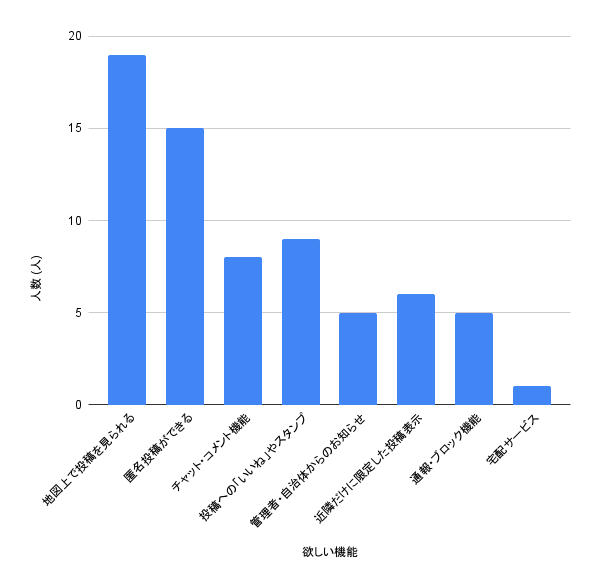
\includegraphics[width=0.5\linewidth]{fig125/Q7.png}
    \caption{欲しい機能}
    \label{fig:Q7}
\end{figure}
図\ref{fig:Q7}より,地域SNSに欲しい機能として地図上での投稿の閲覧,匿名投稿を上げる人が多かった.

\subsection{アンケート結果の分析}
アンケートの結果より土佐山田町に住んでいる人は地域情報を積極的に入手する人は少ないことが分かる.これは,土佐山田町の地域情報を発信している媒体が複数存在しており,情報が分散されていることが原因と考えられる.例として,香美市の公式サイトでは以下の以下の5つの項目を確認できる.
\begin{enumerate}
    \renewcommand{\labelenumi}{・}
    \item くらしの情報
    \item 事業者向け情報
    \item 観光・イベント情報
    \item 市政情報
    \item 施設検索
\end{enumerate}
住民生活に関係するくらしの情報の項目では福祉,税金,交通情報,防災・災害などの18項目を取り扱っている.香美市では以下の6つを公式SNSとして運用している.
\begin{enumerate}
    \renewcommand{\labelenumi}{・}
    \item 香美市公式LINE
    \item 香美市公式Facebook
    \item 香美市立図書館公式Instagram
    \item 香美市あんぱん室(やなせたかし先生顕彰事業推進室)公式Instagram
    \item 香美市消防本部公式Instagram
    \item 香美市山村留学公式Instagram
\end{enumerate}
公式LINEではイベントの情報を中心に,公式Facebookでは活動報告を中心に発信しているInstagramは4つ公式アカウントがあるように分野別にアカウントを分けて発信している.これらの公式SNSに加えて,土佐山田町にある企業や店舗の発信や個人的な発信が様々な媒体で行われている.そのため,必要な情報を得るために複数の媒体を利用しなければならない現状がある.

しかし,アンケートの結果より,地域のイベントの情報や飲食店の情報を求めている人が多く,これらの情報は地図上で投稿が見られるようにするという機能との相性が良いと考えられる.